\chapter{Umsetzung}
In diesem Kapitel werden die wichtigsten Klassen und deren Funktionsweisen erläutert. Jede Klasse wird kurz beschrieben, wobei der Fokus auf ihrer Rolle im Gesamtsystem und ihrer Implementierung liegt.

\section{Klassenübersicht}
Das Klassendiagramm zeigt die Beziehungen der wichtigsten Komponenten des Rubik's Cube Projekts. Die Basis bildet das Interface \texttt{IGameInterface}, das von \texttt{RubiksGameInterface} implementiert wird. Diese zentrale Klasse koordiniert das Zusammenspiel von Eingaben (\texttt{InputSystem}, unterstützt durch \texttt{KeyboardObserver}), der Logik (\texttt{RubiksCube}) und der Darstellung (\texttt{CubieRenderer}).

Der Würfel selbst besteht aus \texttt{Cubie}-Objekten, die von \texttt{RubiksCube} organisiert werden. Zur Unterstützung von Rendering-Aufgaben wird die Klasse \texttt{ShaderUtil} genutzt, welche die Shader-Verwaltung übernimmt. Abbildung \ref{SimpleClassDia} verdeutlicht die Beziehungen der Klassen.

\begin{figure} [H]
	\centering
	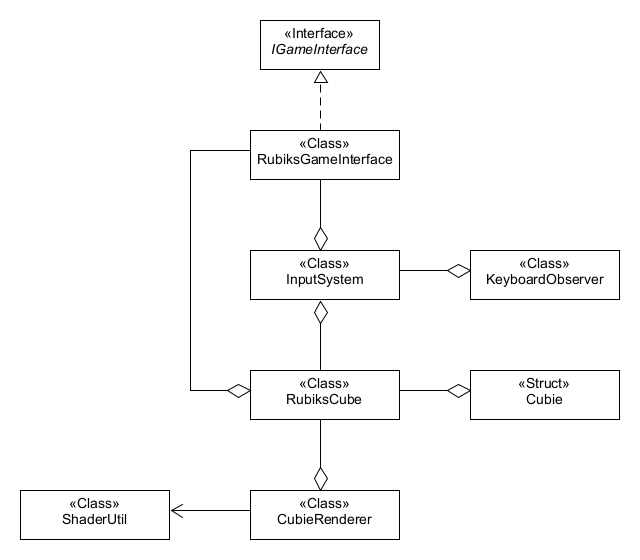
\includegraphics[scale=0.6]{images/SimpleClassDia.png}
	\caption{Vereinfachtes Klassendiagramm}
	\label{SimpleClassDia}
\end{figure}

\section{main.cpp}
Der Code in \texttt{main.cpp} dient als Einstiegspunkt des Projekts. Hier wird \textit{GLFW} initialisiert, ein Fenster erstellt und die \textit{GLEW}-Bibliothek geladen, um moderne OpenGL-Funktionen nutzen zu können. Ein \texttt{RubiksGameInterface}-Objekt wird erstellt und als aktuelle Schnittstelle festgelegt. Der Game-Loop verarbeitet Benutzereingaben und rendert das Fenster. Ein zusätzlicher Mechanismus stellt sicher, dass das Programm bei minimiertem Fenster nicht abstürzt. Nach dem Schließen des Fensters werden mit der Methode \texttt{ShutdownSystem()} alle Ressourcen freigegeben und \textit{GLFW} ordnungsgemäß beendet.


\section{RubiksGameInterface und IGameInterface}
Die Klasse \texttt{RubiksGameInterface} implementiert das Interface \texttt{IGameInterface} und stellt die zentrale Schnittstelle für die Verwaltung des Spiels dar.
Die Methode \texttt{Initialize(GLFWwindow* window)} kümmert sich um die Initialisierung des Spielfensters und des Eingabesystems. Dabei wird das Fensterobjekt in \texttt{m\_window} gespeichert und das Eingabesystem durch den Aufruf von \texttt{m\_input.Initialize(window)} eingerichtet. Der Rubik's Cube wird durch \texttt{m\_rubiksCube.Initialize(*this)} initialisiert. Zusätzlich wird mit \texttt{m\_input.ObserverKey(GLFW\_KEY\_SPACE)} ein Observer für die Leertaste erstellt.

Die Methode \texttt{Render(float aspectRatio)} ist für das Zeichnen des Fensters und des Rubik's Cube verantwortlich. Sie berechnet bei Bedarf die Projektions- und View-Matrizen neu, wenn die Kameraposition oder das Seitenverhältnis des Fensters sich geändert haben. Anschließend wird die Renderlogik auf den Rubik's Cube angewendet, um dessen aktuellen Zustand mit dem Aufruf von \texttt{m\_rubiksCube.Render(m\_projection * m\_view)} darzustellen.

Die Methode \texttt{Update(double deltaTime)} verarbeitet die Benutzereingaben und aktualisiert den Rubik's Cube. Wenn die Leertaste gedrückt wird, erfolgt ein Zurücksetzen des Rubik's Cubes, andernfalls wird \texttt{m\_rubiksCube.Update(*this)} aufgerufen. Änderungen der Kameraentfernung, die durch das Mausrad bedingt sind, werden in Echtzeit aktualisiert, indem der Wert von \texttt{m\_CameraDistance} angepasst wird. Der Kameraabstand wird durch \texttt{if}-Abfragen auf bestimmte Werte begrenzt. Die Methode \texttt{ClearResources()} gibt die Ressourcen des \texttt{m\_rubiksCube}-Objektes frei.

Zusätzlich verfügt die Klasse über die Methode \texttt{QueueMatrixRecalculation()}, die es ermöglicht, das Neuberechnen der Projektions- und View-Matrizen gezielt anzustoßen.
Weitere Getter-Methoden erlauben den Zugriff auf \texttt{m\_deltaTime} und \texttt{m\_input}. 

Abbildung \ref{RubiksGameInterfaceDia} zeigt das Klassendiagramm zu diesem Abschnitt.

\begin{figure} [H]
	\centering
	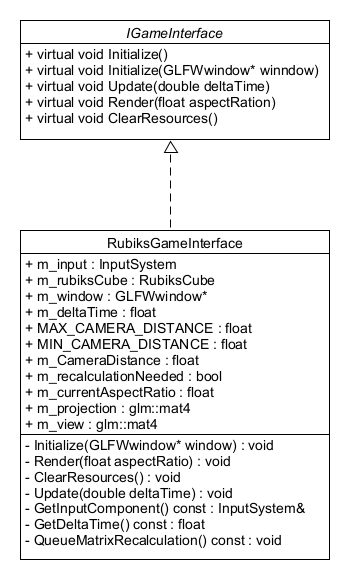
\includegraphics[scale=0.6]{images/GameInterfaceClassDia.png}
	\caption{Klassendiagramm RubiksGameInterface}
	\label{RubiksGameInterfaceDia}
\end{figure}

\section{InputSystem und KeyboardObserver}
Die Klasse \texttt{InputSystem} ist eine zentrale Komponente zur Verwaltung von Benutzereingaben, die sowohl Maus- als auch Tastatureingaben verarbeitet.

Ein zentrales Merkmal des \texttt{InputSystem} ist die Verwaltung der Maustasten-Zustände. Diese werden durch die Enumeration \texttt{ClickState} repräsentiert, die die Zustände \texttt{NO\_ACTION}, \texttt{CLICK}, \texttt{HOLD} und \texttt{RELEASE} definiert. Diese Zustände werden in den Membern \texttt{m\_leftClickState} und \texttt{m\_rightClickState} gespeichert und können über die Methoden \texttt{GetLeftClickState()} und \texttt{GetRightClickState()} abgefragt werden. Dadurch müssen sich andere Klassen nicht um die Details der Zustandsverwaltung kümmern. Zusätzlich wird der aktive Maustasten-Zustand durch die Enumeration \texttt{MouseButton} verwaltet, die die möglichen Maustasten wie \texttt{LEFT\_BUTTON}, \texttt{RIGHT\_BUTTON} und \texttt{NO\_BUTTON} definiert.

Die Aktualisierung der Maustasten-Zustände erfolgt in der \texttt{Update()}-Methode, die regelmäßig aufgerufen wird. Die Methode \texttt{UpdateClickState(MouseButton mouseButton, ClickState\& clickState)} wird dabei verwendet, um den Zustand einer Maustaste basierend auf den aktuellen \textit{GLFW}-Eingaben zu aktualisieren. Dabei wird auch die aktive Maustaste berücksichtigt, um sicherzustellen, dass nicht beide Maustasten gleichzeitig aktiv sind.

Mit den Methoden \texttt{ScreenToWorld(const glm::vec2\& screenPosition)} und \texttt{WorldToScreen(const glm::vec2\& screenPosition)} gibt es auch Möglichkeiten zur Umrechnung zwischen Bildschirmkoordinaten und Weltkoordinaten. Zusätzlich kann mit der Methode \texttt{GetPickingRay(glm::vec3\& out\_origin, glm::vec3\& out\_direction)} ein Strahl erzeugt werden, der in die Richtung der aktuellen Mausposition in die Szene zeigt, um Interaktionen wie das Ziehen von Objekten zu unterstützen.

Die Behandlung des Mausrads erfolgt über eine statische Callback-Funktion \\\texttt{ScrollCallback(GLFWwindow* window, double xScroll, double yScroll)}, \\die von \textit{GLFW} aufgerufen wird, wenn der Benutzer das Mausrad bewegt. Der Scroll-Offset wird in dem statischen Member \texttt{m\_mouseScrollOffset} gespeichert und kann über die Methode \texttt{GetMouseWheelScrollOffset()} abgerufen werden. 

Für die Tastatureingabe wird eine Map von \texttt{KeyboardObserver}-Objekten verwendet, die jeweils den Zustand einer bestimmten Taste verwalten. Der Zustand einer Taste kann über die Methoden \texttt{WasKeyDown(int key)}, \texttt{WasKeyPressed(int key)} und \texttt{WasKeyReleased(int key)} abgefragt werden Die Klasse \texttt{KeyboardObserver} speichert den Zustand einer Taste in den Membern \texttt{m\_wasDown}, \texttt{m\_wasPressed} und \texttt{m\_wasReleased}, die in der \texttt{Update()}-Methode der \texttt{KeyboardObserver}-Klasse aktualisiert werden. 

Eine detaillierte Übersicht der Klassenstruktur ist in Abbildung \ref{InputSystemDia} dargestellt.

\begin{figure} [H]
	\centering
	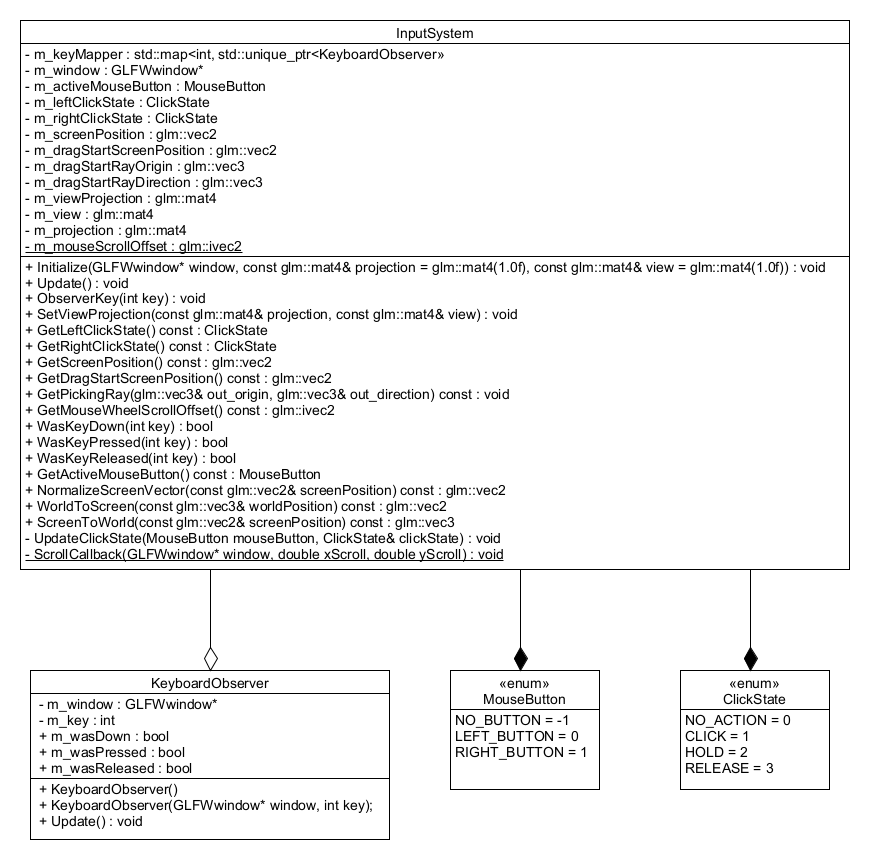
\includegraphics[scale=0.475]{images/InputSystemClassDia.png}
	\caption{Klassendiagramm InputSystem und KeyboardObserver}
	\label{InputSystemDia}
\end{figure}
\newpage
\section{CubieRenderer und ShaderUtil}
Die Klasse \texttt{CubieRenderer} ist für das Rendern der einzelnen Cubies eines Rubik's Cube zuständig. Sie verwaltet die OpenGL-Ressourcen wie Vertex-Buffer, Shader und Texturen, die für die Darstellung der Cubies benötigt werden. Die Initialisierung der Render-Ressourcen erfolgt in der Methode \texttt{Initialize()}, die die Vertex-Daten für die Positionen, Farben und Texturkoordinaten der Cubie-Seiten generiert und in OpenGL-Buffern speichert. Zusätzlich wird ein Shader-Programm geladen, das für die Transformation und das Texturieren der Cubies verantwortlich ist.

Die Methode \texttt{Render(const glm::mat4\& viewProjection, const glm::mat4\& model)} zeichnet einen einzelnen Cubie unter Verwendung der übergebenen Transformationsmatrizen. Die Cubies bestehen aus 36 Vertices, die die sechs Seiten des Würfels repräsentieren. Eine Seite besteht also aus 6 Vertices(zwei Dreiecke). Die Textur wird aktiviert und gebunden, um die Oberfläche der Cubies zu gestalten. Nach dem Rendern werden die OpenGL-Ressourcen wieder freigegeben, um Konflikte mit anderen Render-Operationen zu vermeiden.

Die Klasse \texttt{ShaderUtil} bietet Hilfsfunktionen für das Laden und Kompilieren von Shadern sowie das Laden von Texturen. Dazu gehört \texttt{CreateShaderProgram(const char* vertexFilename, const char* fragmentFilename)}, diese Methode lädt mit \texttt{LoadFile(const char* fileName)} die Vertex- und Fragment-Shader aus Dateien, kompiliert sie und verknüpft sie zu einem Shader-Programm. Dabei auftretende Fehler werden durch die Methoden \texttt{PrintShaderLog(GLuint shader)} und \texttt{PrintProgramLog(GLuint shader)} protokolliert. 

Mit \texttt{LoadTexture(const char* textureFilename)} wird eine 2D-Textur aus einer Bilddatei geladen und die Texturparameter für das Rendering konfiguriert.

Die Struktur und die Beziehungen der Klassen \texttt{CubieRenderer} und \texttt{ShaderUtil} sind detailliert in Abbildung \ref{CubieRendererDia} dargestellt.

\begin{figure} [H]
	\centering
	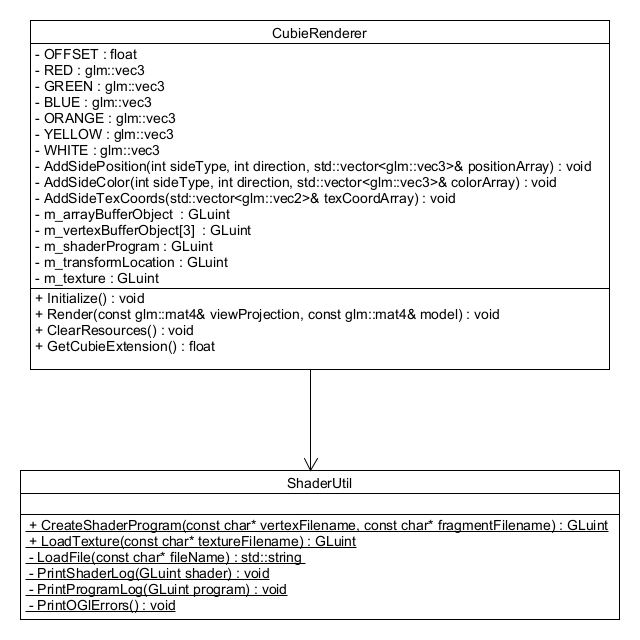
\includegraphics[scale=0.55]{images/CubieRendererClassDia.png}
	\caption{Klassendiagramm CubieRenderer und ShaderUtil}
	\label{CubieRendererDia}
\end{figure}

\section{RubiksCube und Cubie}
